%%%%%%%%%%%%%%%%%%%%%%%%%%%%%%%%%%%%%%%%%
% Programming/Coding Assignment
% LaTeX Template
%
% This template has been downloaded from:
% http://www.latextemplates.com
%
% Original author:
% Ted Pavlic (http://www.tedpavlic.com)
%
% Note:
% The \lipsum[#] commands throughout this template generate dummy text
% to fill the template out. These commands should all be removed when 
% writing assignment content.
%
% This template uses a Perl script as an example snippet of code, most other
% languages are also usable. Configure them in the "CODE INCLUSION 
% CONFIGURATION" section.
%
%%%%%%%%%%%%%%%%%%%%%%%%%%%%%%%%%%%%%%%%%

%----------------------------------------------------------------------------------------
%	PACKAGES AND OTHER DOCUMENT CONFIGURATIONS
%----------------------------------------------------------------------------------------

\documentclass{article}

\usepackage{fancyhdr} % Required for custom headers
\usepackage{lastpage} % Required to determine the last page for the footer
\usepackage{extramarks} % Required for headers and footers
\usepackage[usenames,dvipsnames]{color} % Required for custom colors
\usepackage{graphicx} % Required to insert images
\usepackage{listings} % Required for insertion of code
\usepackage{courier} % Required for the courier font
\usepackage{lipsum} % Used for inserting dummy 'Lorem ipsum' text into the template
\usepackage{pythonhighlight}
\usepackage{siunitx}

% Margins
\topmargin=-0.45in
\evensidemargin=0in
\oddsidemargin=0in
\textwidth=6.5in
\textheight=9.0in
\headsep=0.25in

\linespread{1.1} % Line spacing

% Set up the header and footer
\pagestyle{fancy}
\lhead{\hmwkAuthorName} % Top left header
\chead{\hmwkClass\ : \hmwkTitle} % Top center head
\rhead{\today} % Top right header
\lfoot{\lastxmark} % Bottom left footer
\cfoot{} % Bottom center footer
\rfoot{Page\ \thepage\ of\ \protect\pageref{LastPage}} % Bottom right footer
\renewcommand\headrulewidth{0.4pt} % Size of the header rule
\renewcommand\footrulewidth{0.4pt} % Size of the footer rule

\setlength\parindent{0pt} % Removes all indentation from paragraphs

%----------------------------------------------------------------------------------------
%	CODE INCLUSION CONFIGURATION
%----------------------------------------------------------------------------------------


%----------------------------------------------------------------------------------------
%	DOCUMENT STRUCTURE COMMANDS
%	Skip this unless you know what you're doing
%----------------------------------------------------------------------------------------

%----------------------------------------------------------------------------------------
%	NAME AND CLASS SECTION
%----------------------------------------------------------------------------------------

\newcommand{\hmwkTitle}{Predicting Boston Housing Prices} % Assignment title
\newcommand{\hmwkDueDate}{January\ 25,\ 2016} % Due date
\newcommand{\hmwkClass}{MLE Nanodegree \#1} % Course/class
%\newcommand{\hmwkClassTime}{10:30am} % Class/lecture time
%\newcommand{\hmwkClassInstructor}{Jones} % Teacher/lecturer
\newcommand{\hmwkAuthorName}{Ilan Stefanon} % Your name

%----------------------------------------------------------------------------------------
%	TITLE PAGE
%----------------------------------------------------------------------------------------

\title{
\vspace{2in}
\textmd{\textbf{\hmwkClass:\ \hmwkTitle}}\\
\normalsize\vspace{0.1in}\small{Due\ on\ \hmwkDueDate}\\
\vspace{0.1in}\large{\textit{\hmwkClassInstructor\ \hmwkClassTime}}
\author{\textbf{\hmwkAuthorName}}
\date{\today}
\vspace{3in}
}

%----------------------------------------------------------------------------------------

\begin{document}

\maketitle

%----------------------------------------------------------------------------------------
%	TABLE OF CONTENTS
%----------------------------------------------------------------------------------------

%\setcounter{tocdepth}{1} % Uncomment this line if you don't want subsections listed in the ToC

\newpage
\tableofcontents
\newpage

%----------------------------------------------------------------------------------------
%----------------------------------------------------------------------------------------



\section{Statistical Analysis and Data Exploration}

The dataset has the following characteristics : 

\begin{description}
\item[Number of data points :] 506
\item[Number of features :] 13
\item[Minimum and maximum housing prices :] 5 to 50 (thousands of dollars)
\item[Mean and median Boston housing prices :] 22.5 and 21.2
\item[Standard deviation :] 9.2
\end{description}

The number of data points is relatively small. We'll have to take into account this when we'll split the data into training/testing set. The testing set should not be too small.
The standard deviation is not too big if we compare it to the minimum and maximum housing prices. It means that there is not a lot of dispersions ( not too much outliers). We'll don't have to clean the data.

%----------------------------------------------------------------------------------------
%----------------------------------------------------------------------------------------

\section{Evaluating Model Performance}

Several model performance is possible with regression : 
 
\begin{itemize}
\item Mean Absolute Error (MAE). Easiest regression metric to understand. It assigns equal weight to the data.
\item Mean Squared Error (MSE). This metric "`punishes"' larger errors (outliers) and is useful in the real world.
\item Coefficient of determination(R squared). It's a rescaling of MSE.
\item Root Mean Squared Error (RMSE). It's close to MSE, with the advantage to represent a real value(thousands dollars).
\end{itemize}
In our case, we'll use the standard metric RMSE. It makes an excellent general purpose metric.

\par It's important to split the data into training and testing data to be able to predict future data. Maximizing training performance only will cause overly complex model that won't generalize to new data. For this reason, it should use a testing data to estimate the model trains by the train data. 
\par But train/test split will provide a high variance estimate since changing which data to be in train/test bag can change the performance of the model. So is even better to create several train/test splits under the same data and average the results together. It's the goal of the cross-validation.
\par I have used \pyth{cross_validation.train_test_split( X, y, test_size=0.4, random_state=0)}.
I choose the test size to \num{33} percent of the total size to be sure to don't have too high variance on the test set.
Finally, the model used (decision trees) for regression provided Scikit-learn  is a function with several parameters. To be able to find the best combination of parameters it's possible to use Grid search. It's an approach to tune the parameters automatically. It methodically builds and evaluate the model for each combination of parameters specified in a grid. In this project, only max_depth is tuned.

%----------------------------------------------------------------------------------------

\section{Analyzing Model Performance}


When there are very few training examples it's very easy to fit every single one training example so near the origin the error is small and when the training size increase it's harder to fit perfectly and the training set error is larger and larger. About the test error, with few training set we don't generalize well so will get a high error. With larger training set were are able to generalize depending on the quality of the model. so the test error decrease.

If we have high a bias(underfitting), if we increase the size of the training set we still underfit the data so the test error will decrease but the error will still be high with any size of the training set. the training error will begin low and will increase and will end up close the test error because with so few parameters the performance on the training set and test set will be very close. If we have a learning algorithm with high bias, getting more training data will not help much. Such behavior is characteristic of the learning curve with maximum depth equal to 1 as shown in the following Figure \ref{learning_curve_1}.

\begin{figure}[h]
  \begin{center}
	\caption{\label{learning_curve_1} Learning curve maximum depth = 1}
	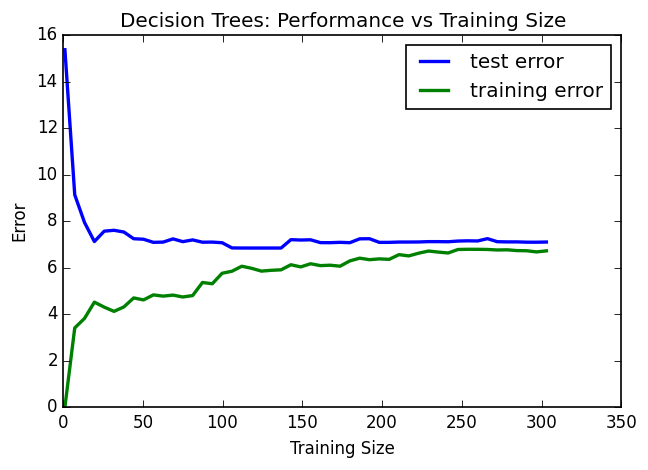
\includegraphics[width=0.75\columnwidth]{learning_curve_depth_1} % Example image
	\end{center}
\end{figure}


If we have high variance (overfitting), we'll have a training error that  will be small with few data and  we still have a low training error (just a bit higher) with a larger data set. Regarding the test error, it will decrease with the increasing of the training set but there  will be a large gap between training error and test error. Getting more training data is likely to help to decrease the test error. the following figure \ref{learning_curve_10} show a model with quite high-variance estimator. Increasing the training sizes could lead to better generalization performance.

\begin{figure}[h]
  \begin{center}
	\caption{\label{learning_curve_10} Learning curve maximum depth = 10}
	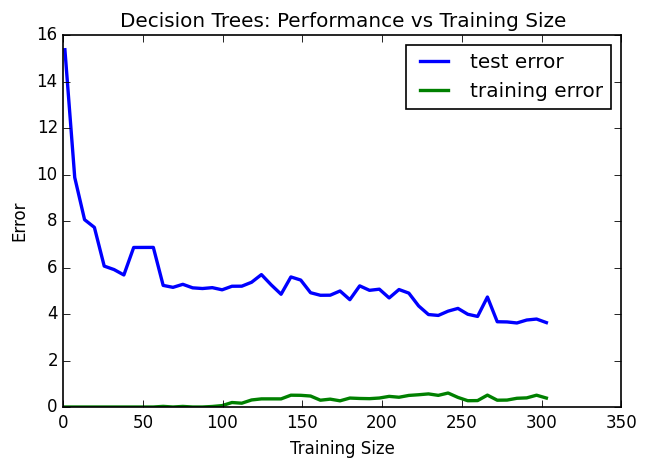
\includegraphics[width=0.75\columnwidth]{learning_curve_depth_10} % Example image
	\end{center}
\end{figure}

The figure \ref{complexity_graph} represents the complexity graph which is the evolution of the error vs increase of the max depth (complexity) in our project. It appears that the bias is reduced to almost zero for maximum depths greater than  \num{10} but the variance term is not reduced further after the max depth  \num{5} is reached. The optimal model complexity seems to be around a maximum depth of \num{6} to \num{10}. 


\begin{figure}[h]
  \begin{center}
	\caption{\label{complexity_graph} Complexity graph}
	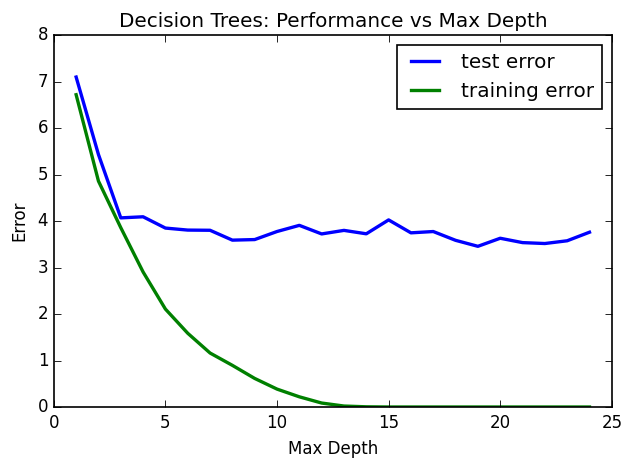
\includegraphics[width=0.75\columnwidth]{complexity_graph} % Example image
	\end{center}
\end{figure}


\section{Model Prediction}

As explained in the section Evaluating Model Performance, we used root mean squared error as performance metric : 
\inputpython{boston_housing_students.py}{181}{183}

\pyth{GridSearchCV} as been parametrized like this : 

\pyth{GridSearchCV(regressor, param_grid=parameters,scoring=rmse_scorer, cv=3)}

We used a cross-validation generator of 3-fold. It correspond approximately to the test size of 0.4 used in the learning curve.

\pyth{GridSearchCV} found the best $\texttt{max\_depth} = 10$ with a corresponding RMSE of 5.878.

The prediction computed is 20.72 thousand of dollars.

\end{document}